\documentclass[twoside,twocolumn]{ujarticle}
%\usepackage{type1cm}
\usepackage{outline-ec}
\usepackage{amsmath,amssymb,verbatim,ascmac,multicol}
\usepackage{tabularx}
% dvioutで確認する場合は以下を有効にする
%\usepackage[dviout]{graphicx,color}
% pdf化する場合は以下を有効にする
\usepackage[dvipdfmx]{graphicx,color}



%
% --------------------------------------------------------------------------
% 本文開始
%
\begin{document}

\twocolumn[
\begin{center}
  {\large \bf キーボード打鍵時の手指動画像を用いた継続認証方法の検討---研究方針}
  \par
  \vspace{5mm}
  {\normalsize 長谷川 颯一}
  \vspace{3mm}
\end{center}
\vspace{5mm}
]

%
% --------------------------------------------------------------------------
% 第1節
%
\section{先行研究}
%
本研究は，Rothらの研究「On Continuous User Authentication via Typing Behavior」を基に進める．
この研究の概要を以下に簡単にまとめる．

\subsection{提案された手法}

\noindent \textbf{特徴量の抽出}

Rothらは，各フレームから左右の手の特徴を抽出している．
LDAによって手指領域の検出を行い，以下の2種類の特徴量を抽出している．
\begin{enumerate}
  \setlength{\parskip}{0cm}
  \setlength{\itemsep}{0cm}
  \item Shape Context：手の輪郭形状を表す特徴量
  \item Centroid：手の領域の重心位置
\end{enumerate}
Shape Contextは，手の輪郭を，重心を中心とした3つの同心円と12の角度方向に分割し，
各領域に含まれる輪郭点の分布をヒストグラムで表現する．
以上より，1フレームは76次元の特徴記述子で表現される．

この特徴記述子に対し，Bag of Words（BoW），Bag of Phrases（BoP），Bag of Multi-dimensional Phrases（BoMP）の3種類の特徴表現を行い，
それぞれの特徴表現に基づいて動画間の類似度を算出している．

\vspace{0.2cm}
\noindent \textbf{BoW}

BoWは，本研究の中間発表で検証した手法である．
抽出した特徴量を，k-means法によってクラスタリングし，各フレームの特徴量を最も近いコードワードに割り当てる．
その後，動画中の各コードワードの出現回数をカウントし，正規化することでヒストグラムを得る．
登録映像と認証映像のヒストグラムの内積を算出することで，動画間の類似度が得られる．

\vspace{0.2cm}
\noindent \textbf{BoP}

BoWには，時間的な情報が失われるという欠点がある．
この問題を改善するために検討されたのがBoPである．
BoPでは，単独のコードワードだけでなく，コードワードの出現順序や時間的な配置関係を考慮する．
これにより，単なるコードワードの出現頻度だけでなく，コードワードの出現パターンを特徴量として利用できる．
しかし，BoWやBoPでは，左手の形状や動きが一致していても，右手のそれらが一致していない場合に違うコードワードに割り当てられてしまい，
この一致が類似度に反映されない可能性がある．

\vspace{0.2cm}
\noindent \textbf{BoMP}

この問題を改善するために検討されたのがBoMPである．
BoMPでは，次の4種類のコードブックを作成する．
\begin{enumerate}
  \setlength{\parskip}{0cm}
  \setlength{\itemsep}{0cm}
  \item 左手のShape Contextのコードブック
  \item 左手のCentroidのコードブック
  \item 右手のShape Contextのコードブック
  \item 右手のCentroidのコードブック
\end{enumerate}
BoPでは，これらを1つのコードブックにまとめていたが，BoMPではそれぞれのコードブックを独立して扱う．
そのため，例えば左手の形状が一致し，右手の形状が一致しない場合でも，一致した特徴量の情報を類似度に反映できると考えられる．

\subsection{実験と結果}

Rothらは，63人の被験者を対象に，固定文章・自由文章を入力した際のデータを収集した．
前節で述べた3種類の特徴表現を用いた場合の認証性能を比較した結果，BoMPが最も高い認証性能を示した．
\begin{table}[htbp]
  \centering
  \caption{BoW，BoP，BoMPの認証性能比較}
  \label{tab:BoW_BoP_BoMP}
  \begin{tabular}{c|ccc}
    \hline \hline
    手法 & AUC & TPR0 & FPR0 \\
    \hline
    BoW  & 0.9934 & 6.9 & 21.5 \\
    BoP  & 0.9937 & 13.6 & 21.7 \\
    BoMP & 0.9975 & 27.4 & 4.3 \\
    \hline \hline
  \end{tabular}
\end{table}
TPR0は，FPRが$0.001\%$のときのTrue Positive Rate
（他人を誤って本人と判定する確率を$0.001\%$に抑えた場合に，本人を正しく本人と判定できる割合）を表す．
FPR0は，TPRが$99\%$のときのFalse Positive Rate
（本人を正しく本人と判定する確率を$99\%$にした場合の，他人を誤って本人と判定する割合）を表す．

さらに，パラメータ$L$（連結フレーム数）と$D$（コードワード数）を変化させた場合の認証性能の比較も行っている．
連結フレーム数については，$L = 4$のときに最も高い認証性能が得られ，
コードワード数については，$D \approx 400$付近で性能が飽和した．

他にも，
\begin{itemize}
  \setlength{\parskip}{0cm}
  \setlength{\itemsep}{0cm}
  \item 登録した動画・認証対象の動画の長さが長いほど，認証性能が向上する傾向があること
  \item 静的特徴のみを用いた場合よりも高い認証性能が得られたこと
  \item BoMPの認証性能は，キーストロークダイナミクスを用いた認証手法よりも高いこと
\end{itemize}
が報告されている．

%
% --------------------------------------------------------------------------
% 第2節
%
\section{本研究の方針}
%

\subsection{課題の検討と目的の設定}

中間発表では，特徴量にMediaPipeを用いたBoWの検証を行った．
5人の被験者を対象に，固定文章を打鍵した際のデータを収集して類似度を算出した．
その結果，同一被験者間の類似度は高く，異なる被験者間の類似度は低くなる傾向が確認され，
MediaPipeを用いた場合でも，BoWによって個人特有の特徴を抽出することができる可能性が示唆された．

これまでの取り組みや，中間発表での質疑から，現状では以下のような課題があると考えられた．\\

\noindent \textbf{認証性能に関する課題}
\begin{itemize}
  \setlength{\parskip}{0cm}
  \setlength{\itemsep}{0cm}
  \item BoWの認証性能の評価
  \item BoP，BoMPの認証性能の評価
  \item パラメータ$D$，$L$の最適化
  \item 被験者を増やした場合の検証
\end{itemize}
\textbf{条件変化に関する課題}
\begin{itemize}
  \setlength{\parskip}{0cm}
  \setlength{\itemsep}{0cm}
  \item キーボードやカメラの位置・種類の違い
  \item 撮影日時の違い  
  \item マウス利用も撮影に含めた場合の検証
\end{itemize}
\textbf{実用性に関する課題}
\begin{itemize}
  \setlength{\parskip}{0cm}
  \setlength{\itemsep}{0cm}
  \item 打鍵に慣れていない被験者の検証
  \item Rothらの手法との比較
  \item 攻撃に対する耐性の検証
\end{itemize}

重要な課題を整理し，本研究の中心的な問いを
「\emph{特徴量にMediaPipeを用いた場合のBoW，BoP，BoMPの認証性能はどの程度か}」とする．
実用化を考える上では，キーボードやカメラのずれや種類の違い，日時の違いなどの条件変化に対する頑健性も重要であるが，
まずはそれらの条件変化がない場合における認証性能を明らかにすることを優先する．

\subsection{実験の計画}

前節で設定した問いを軸として，以下の順に実験を進めていく．
\begin{enumerate}
  \setlength{\parskip}{0cm}
  \setlength{\itemsep}{0cm}
  \item BoWを用いた場合の認証性能の評価
  \item BoPを用いた場合の認証性能の評価
  \item BoMPを用いた場合の認証性能の評価
  \item 3手法の認証性能の比較
\end{enumerate}

まずは，以下のような条件で撮影を行う．
\begin{table}[htbp]
  \setlength{\intextsep}{0cm}    % [h]指定などの表の前後を詰める
  \centering
  \begin{tabular}{ll}
    項目 & 条件 \\
    \hline
    被験者 & 電子制御工学科5年生の学生 全員？ \\
    撮影回数 & 1人あたり5回 \\
    入力文章 & 固定文章$\times$4種類・自由文章$\times1$ \\
    文章の長さ & $40 \sim 50$words程度 \\
    カメラ & Webカメラ (SmartCam C960 AF) \\
    FPS & 30fps \\
    カメラ位置 & 固定 \\
    キーボード & 固定
  \end{tabular}
\end{table}
\begin{description}
  \setlength{\parskip}{0cm}
  \setlength{\itemsep}{0cm}
  \item[固定文章] 英文4種類を用意し，全被験者に同じ文章を入力してもらう．
  \item[自由文章] お題を設定し，Microsoft Wordを使用して日本語または英語で自由に文章を入力してもらう．  
\end{description}

撮影した動画は，学習用(training)・検証用(validation)・テスト用(test)に分割して使用する．
検証用の動画は，登録用（enrollment）・認証用（probe）に分ける必要がある．
テストでは，検証時に作成した登録情報と認証閾値を使用するため，認証対象（probe）の動画のみを用いる．
固定文章の4本の動画は以下のようなフォルダに分けて保存し，
自由文章の動画は追加評価に用いる．
\begin{itemize}
  \setlength{\parskip}{0cm}
  \setlength{\itemsep}{0cm}
  \item \verb|data/training/|
  \item \verb|data/validation/enrollment/|
  \item \verb|data/validation/probe/|
  \item \verb|data/test/probe/|
\end{itemize}

取得した動画を，図\ref{fig:flow}に示すような流れで処理する．
学習では，training内の動画を用いてBoW，BoP，BoMPのコードブックを構築する．
登録では，validation/enrollment内の動画を用いて個人ごとの特徴表現を作成し，
validation/enrollmentとvalidation/probeの動画間の類似度を算出して認証閾値を決定する．
最終評価では，登録した特徴表現とtest/probeの動画との類似度を算出し，
検証で決定した閾値を用いて認証性能を評価する．
BoMPについては，左手と右手のコードブックを作成し，それぞれの類似度を算出した後に平均をとることで最終的な類似度を算出する．
\begin{figure}[htbp]
  \centering
  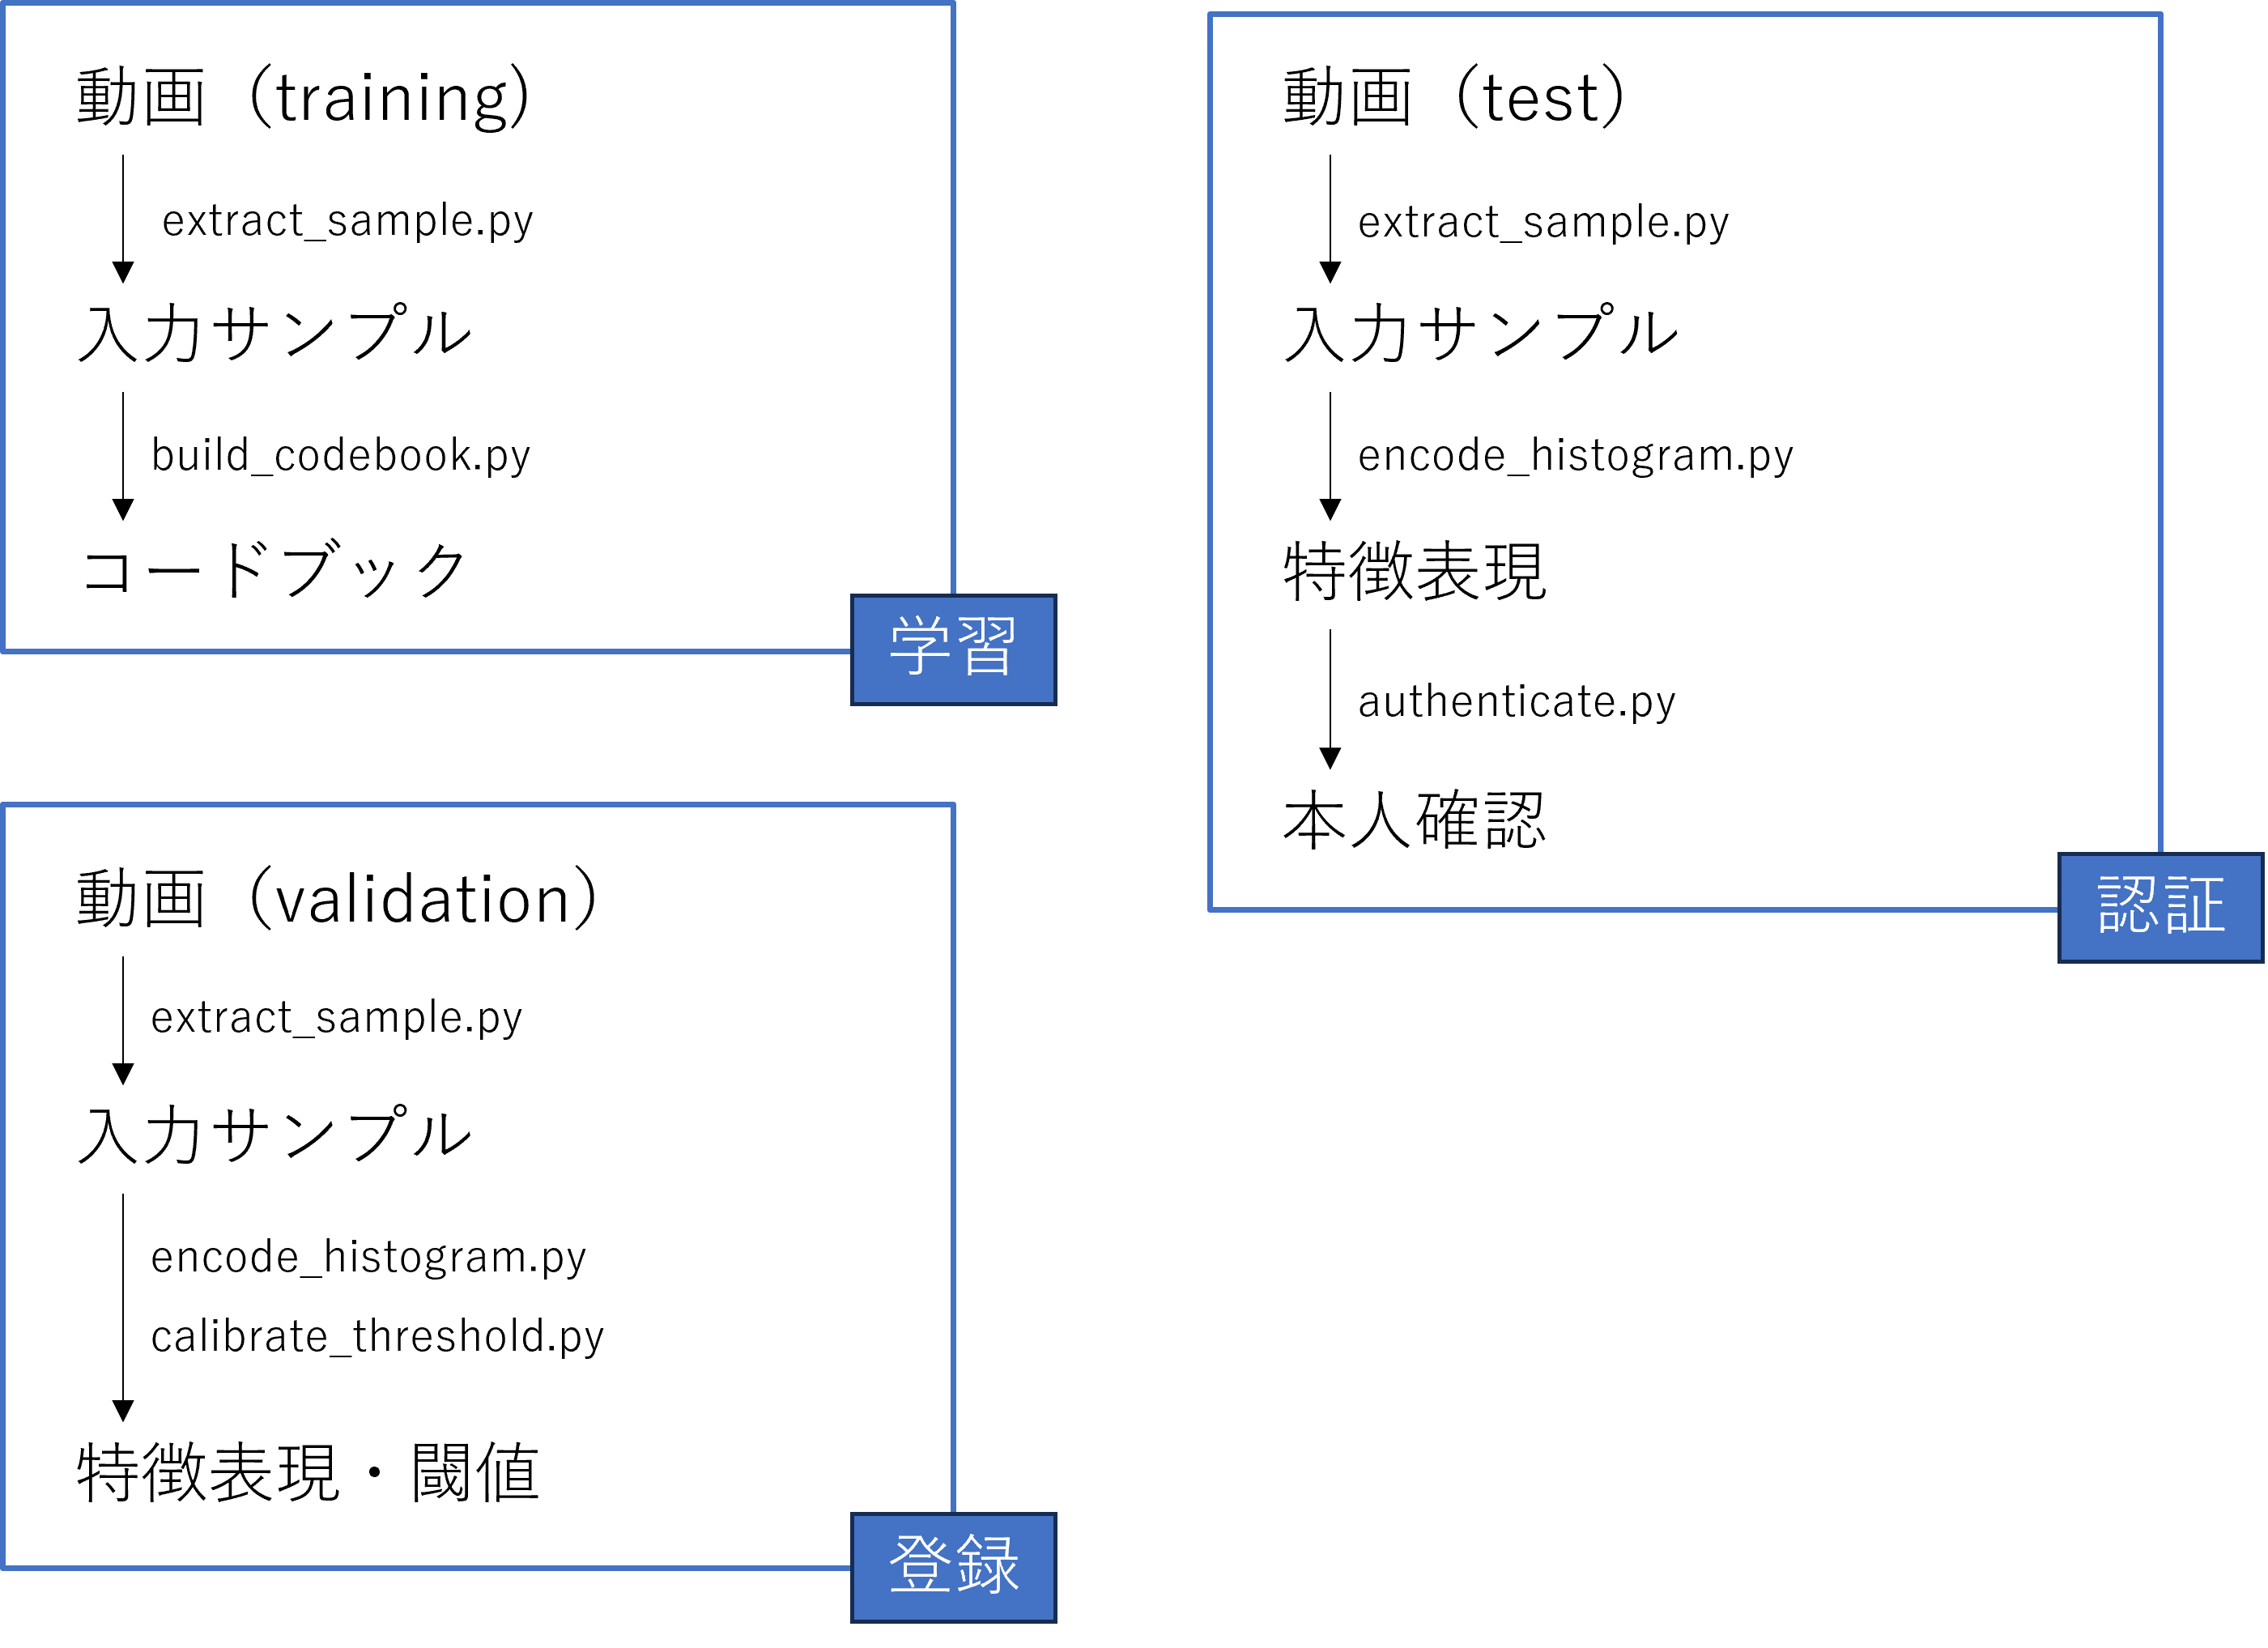
\includegraphics[width=0.45\textwidth]{programs.png}
  \caption{動画処理の流れ}
  \label{fig:flow}
\end{figure}

評価指標として以下を用いる．
\begin{itemize}
  \setlength{\parskip}{0cm}
  \setlength{\itemsep}{0cm}
  \item EER(Equal Error Rate)：FARとFRRが等しくなる点の値
  \item AUC(Area Under Curve)：ROC曲線の下の面積
  \item TPR0：FPRが$0.001\%$のときのTrue Positive Rate
  \item FPR0：TPRが$99\%$のときのFalse Positive Rate
\end{itemize}

11月から12月頭にかけて撮影を行い，12月中旬までにBoWの認証性能を評価する．
年内にはBoPとBoMPの認証性能を評価し，3手法の認証性能を比較する．
余裕があれば，自由文章を入力している際の動画を用いた評価や，
日時が変わった際の認証性能の評価，攻撃に対する耐性の検証も行う．

\end{document}
